\documentclass[10pt,conference]{IEEEtran}
\usepackage{amsmath,amssymb}
\usepackage{booktabs}
\usepackage{graphicx}
\usepackage{xcolor}

\newcommand{\method}{SwiftPose-Fi}

\title{\method: Decomposition-Guided Fast Inference for Hardware-Friendly Wi-Fi Human Pose Estimation}

\author{
\IEEEauthorblockN{Toan D. Gian}
\IEEEauthorblockA{TODO: affiliation\\
TODO: email}
}

\begin{document}
\maketitle

\begin{abstract}
Wi-Fi human pose estimation (HPE) enables camera-free sensing, but current Wi-Fi HPE systems remain difficult to deploy on tiny edge devices because they feed entangled channel state information (CSI) into neural networks and rely on the model to internally discover pose-relevant structure. This paper argues that practical Wi-Fi HPE requires a different system abstraction: first decompose CSI into physically meaningful components, then use a small hardware-friendly model to selectively fuse those components. We present \method, a decomposition-guided Wi-Fi HPE system for fast inference on edge devices. \method\ factorizes each CSI frame into link, subcarrier, and packet factors using non-negative CP decomposition, and estimates pose using selective component-adaptive fusion (S-AFF). CP exposes interpretable wireless components, while S-AFF provides a compact deployable neural predictor that chooses, per sample, whether pose should be predicted from one dominant component or from a fused component representation. A sharpening loss encourages decisive sparse gates rather than uninformative near-uniform averaging. On the full MM-Fi protocol-3 frame-level split with 320,760 CSI frames, CP+S-AFF achieves 50.80\% PCK$_{20}$ with only 64.9K parameters and about 2.89M FLOPs per frame. Compared with HPE-Li, a strong lightweight Wi-Fi HPE baseline with 1.66M parameters and 2.42G FLOPs, CP+S-AFF reduces parameters by 26$\times$ and FLOPs by more than 838$\times$ while remaining within 1.27 PCK$_{20}$ points. We further adapt the decomposition principle to Person-in-WiFi 3D by using a lightweight query S-AFF head and, for the single-person setting, separate amplitude and phase CP streams. On true single-person Person-in-WiFi 3D, dual-stream CP+S-AFF reaches 83.82 mm MPJPE with 1.70M parameters, outperforming the original 48.2M-parameter Person-in-WiFi 3D baseline but still trailing the recent 2.14M-parameter WiFi-Mamba result; a 923K-parameter profile approximately matches the original Person-in-WiFi 3D baseline with 52.2$\times$ fewer parameters. Component ablation shows that removing one decomposed component causes up to an 18.94-point PCK$_{20}$ drop, and removing the subcarrier factor causes a 24.90-point drop. These results show that decomposition is not merely compression: it exposes pose-relevant CSI structure and creates a hardware-friendly bridge from Wi-Fi HPE algorithms to real edge deployment.
\end{abstract}

\section{Introduction}

Wi-Fi sensing has become an attractive alternative to camera-based perception because it reuses existing wireless infrastructure and preserves visual privacy. In particular, Wi-Fi human pose estimation (HPE) aims to recover body keypoints from channel state information (CSI), enabling fine-grained sensing without cameras or wearable devices. Recent Wi-Fi HPE systems show that CSI contains rich pose information, and methods such as Person-in-WiFi~\cite{personwifi2019}, GoPose~\cite{gopose2021}, MetaFi~\cite{metafi2022}, Person-in-WiFi 3D~\cite{personwifi3d2024}, WiFi-Mamba~\cite{wifimamba2026}, GraphPose-Fi~\cite{graphposefi2026}, MultiDim-Fi~\cite{multidimfi2025}, and HPE-Li~\cite{hpeli2024} demonstrate strong progress in wireless pose estimation.

However, a gap remains between accurate Wi-Fi HPE simulation and practical real-world deployment. Most existing systems follow a direct neural inference pipeline: transform CSI into amplitude, phase, image-like, spectrum-like, or sequence-like inputs, and train a neural model to estimate pose. This approach can be accurate, but it forces the neural network to solve two tasks at once: separate pose-relevant wireless structure from entangled CSI, and map that structure to keypoints. When deployed on resource-constrained hardware such as Raspberry Pi or Jetson Nano, this coupling is expensive. A model that internally learns signal decomposition often needs more parameters, more FLOPs, and more memory than a tiny edge device can comfortably support.

\textbf{Our position is simple: Wi-Fi HPE should decompose before learning.} Raw CSI is not a clean observation of human pose. It is a superposition of static paths, human reflections, device responses, frequency-selective fading, packet-level variation, and noise. Instead of asking a neural network to discover this structure implicitly, \method\ explicitly decomposes the CSI tensor into compact physical factors, then feeds those factors to a small component-adaptive fusion model.

This creates a system architecture with two practical advantages. First, the decomposition stage reduces and organizes the input: a frame with $3\times114\times10=3420$ CSI values becomes a 508-dimensional component representation. Second, the predictor becomes hardware-friendly: S-AFF uses dense layers, lightweight convolutions, and a sparse softmax gate, all of which can be exported to standard neural runtimes such as TorchScript, ONNX Runtime, TensorRT, or CPU-optimized kernels. This is fundamentally more deployable than large neural backbones or tree ensembles with millions of branch nodes.

The key technical question is whether decomposed CSI components are actually useful for HPE. Our full-MM-Fi results answer yes. Under the same predictor family, CP components improve nonlinear prediction over raw-statistic features. CP+S-AFF reaches 50.80\% PCK$_{20}$ with 64.9K parameters. CP+CNN reaches 49.62\% PCK$_{20}$ with 77.6K parameters. CP+ExtraTrees reaches 50.40\% PCK$_{20}$, close to HPE-Li's reported 52.07\%, but is not deployment-friendly and is used only as an analysis baseline. Most importantly, ablation shows that decomposed components are not cosmetic: removing the strongest component drops PCK$_{20}$ by 18.94 points.

This paper makes the following contributions:
\begin{itemize}
    \item We introduce a decomposition-guided Wi-Fi HPE system architecture designed for fast inference and edge deployment.
    \item We formulate CSI frame decomposition using non-negative CP factorization, exposing link, subcarrier, and packet factors.
    \item We design selective component-adaptive fusion (S-AFF), a tiny neural predictor that preserves single-factor experts, includes a fused-factor expert, and uses a sharpened per-sample gate to route each input.
    \item We evaluate on the full MM-Fi protocol-3 frame-level split using the HPE-Li PCK metric and add a cross-dataset adaptation study on Person-in-WiFi 3D.
    \item We show that CP+S-AFF reduces parameters by 26$\times$ and FLOPs by more than 838$\times$ compared with HPE-Li while staying within 1.27 PCK$_{20}$ points.
    \item We analyze deployment friendliness through operator portability, model size, latency bottlenecks, and controllable CP rank/iteration knobs.
    \item We provide component and factor-mode ablations showing that decomposed factors carry pose-relevant information.
\end{itemize}

\section{Design Goals}

\method\ is designed around four systems goals.

\textbf{G1: Separate signal organization from pose prediction.}
Raw CSI is an entangled physical measurement. A deployable system should not require a large neural model to discover all wireless structure implicitly. \method\ explicitly decomposes CSI before prediction.

\textbf{G2: Preserve physically meaningful modes.}
CSI is naturally multi-way: links capture spatial visibility, subcarriers capture frequency-selective multipath, and packets capture short-time dynamics. A useful representation should preserve these modes instead of flattening them too early.

\textbf{G3: Keep the predictor hardware-friendly.}
A practical edge model should consist of operations that map well to embedded runtimes. Dense layers, lightweight convolutions, pooling, and softmax gates are friendly to ONNX Runtime, TensorRT, TorchScript, CPU vectorization, and micro-batching.

\textbf{G4: Provide component-level evidence.}
If decomposition is the main contribution, accuracy alone is insufficient. We must show that the decomposed factors are actually used by the predictor. Therefore, \method\ evaluates component ablation and factor-mode ablation in addition to PCK.

\section{Background and Motivation}

\subsection{CSI as a Mixed Wireless Signal}

CSI over frequency $f$ and time $t$ can be modeled as a multipath superposition:
\begin{equation}
H(f,t)=\sum_{q=1}^{Q}\alpha_q(t)e^{-j2\pi f\tau_q(t)}+n(f,t),
\end{equation}
where $\alpha_q(t)$ is the complex path attenuation, $\tau_q(t)$ is the path delay, and $n(f,t)$ is noise. Human motion changes only part of this mixture. Static reflectors, line-of-sight propagation, device response, and hardware noise remain entangled with human-induced paths.

For HPE, this mixture is especially challenging. A keypoint does not correspond to one subcarrier or one packet. Body geometry affects CSI through distributed multipath patterns across links, subcarriers, and time. Therefore, a direct model must implicitly learn how to separate and aggregate wireless factors before estimating pose.

\subsection{Why Direct Neural HPE Is Hard to Deploy}

Let $X\in\mathbb{R}_{+}^{L\times S\times P}$ be a CSI frame, where MM-Fi uses $L=3$ links, $S=114$ subcarriers, and $P=10$ packets. Direct Wi-Fi HPE learns
\begin{equation}
\hat{y}=F_\theta(X),
\end{equation}
where $y\in\mathbb{R}^{17\times3}$ is the target pose. The neural model $F_\theta$ must learn both wireless representation and pose mapping. This is acceptable in a server setting, but it is expensive on tiny devices. HPE-Li~\cite{hpeli2024} reduces this burden with a lightweight neural design, yet still uses 1.66M parameters and 2.42G FLOPs. Our goal is not merely to compress a neural model, but to change the signal abstraction so the predictor itself can be tiny.

\section{Related Work}

\textbf{Wi-Fi human pose estimation.}
Person-in-WiFi~\cite{personwifi2019} showed that Wi-Fi can support fine-grained person perception. GoPose~\cite{gopose2021} and Person-in-WiFi 3D~\cite{personwifi3d2024} further explored 3D human pose estimation from commodity Wi-Fi using amplitude, phase, and spatial-spectrum representations. WiFi-Mamba~\cite{wifimamba2026} recently showed that separating amplitude and phase streams and using efficient state-space sequence modeling can substantially improve Person-in-WiFi 3D accuracy with far fewer parameters than the original transformer baseline. MetaFi~\cite{metafi2022} demonstrated device-free pose estimation and reports strong PCK@50 on its own setup. HPE-Li~\cite{hpeli2024} is the most relevant direct baseline because it targets lightweight Wi-Fi HPE and reports MM-Fi protocol results with the same PCK family used in our evaluation. More recent methods such as GraphPose-Fi~\cite{graphposefi2026} and MultiDim-Fi~\cite{multidimfi2025} explore graph or transformer-style modeling on MM-Fi, but their reported settings are not always directly comparable to the HPE-Li frame-level protocol3 split used here.

\textbf{Lightweight wireless sensing.}
Efficient Wi-Fi sensing has been studied for activity recognition, gesture recognition, and compression. EfficientFi~\cite{efficientfi2023} and LiteHAR~\cite{litehar2022} show that lightweight CSI processing can reduce deployment cost, while SenseFi~\cite{sensefi2023} provides benchmark infrastructure for Wi-Fi sensing models. These works motivate efficiency, but HPE is more demanding than classification because the model must recover a structured set of body keypoints.

\textbf{CSI decomposition and fusion.}
WiDeFus~\cite{widefus2026} is closest in spirit. It extracts human-path CSI components and uses adaptive feature fusion for lightweight activity recognition. \method\ differs in task, representation, and evaluation. Instead of classifying activities from a purified phase component, \method\ estimates 17 human keypoints from multiple CP factors and evaluates whether each factor contributes to pose prediction. We adapt the fusion principle of WiDeFus to link, subcarrier, and packet factors.

\textbf{Tensor decomposition.}
Tensor factorization has a long history in multi-way signal analysis~\cite{kolda2009}. CP decomposition is attractive for CSI because it decomposes a tensor into rank-one components while preserving modal structure. Tucker decomposition is more expressive but introduces a core tensor that complicates interpretation. Matrix factorization loses modal structure by flattening. \method\ uses CP because it is compact, interpretable, and implementation-friendly.

\section{Problem Formulation}

Let $\mathcal{D}=\{(X_i,y_i)\}_{i=1}^{N}$ be a Wi-Fi HPE dataset where $X_i\in\mathbb{R}_{+}^{L\times S\times P}$ is one CSI frame and $y_i\in\mathbb{R}^{17\times3}$ is the corresponding pose. A direct neural method learns
\begin{equation}
\theta^\star=\arg\min_\theta \sum_i \ell(F_\theta(X_i),y_i),
\end{equation}
where $F_\theta$ must jointly learn signal representation and pose mapping.

\method\ instead solves
\begin{equation}
\phi^\star,\omega^\star=
\arg\min_{\phi,\omega}\sum_i
\ell(G_\omega(D_\phi(X_i)),y_i),
\end{equation}
subject to a deployment budget
\begin{equation}
\mathrm{Params}(G_\omega)+\mathrm{Ops}(D_\phi,G_\omega)\leq B.
\end{equation}
This formulation makes the systems objective explicit: retain pose accuracy while reducing the cost of the deployed feature extractor and predictor.

\section{System Overview}

\method\ uses a two-stage pipeline:
\begin{equation}
X \xrightarrow[]{D_\phi} Z=(A,B,C) \xrightarrow[]{G_\omega^{S\text{-}AFF}} \hat{y}.
\end{equation}
The decomposition module $D_\phi$ extracts physical CSI factors. The fusion module $G_\omega^{S\text{-}AFF}$ selectively fuses these factors for pose estimation.

\textbf{Edge execution.}
At runtime, the edge device receives CSI frames, normalizes amplitude values, applies CP decomposition, forms the compact factor vector, and runs S-AFF to predict pose. The pipeline operates on one frame at a time, matching the HPE-Li frame-level protocol. This design avoids transmitting raw CSI to a server and avoids running a large HPE network locally.

\textbf{Why not deploy ExtraTrees?}
ExtraTrees performs well in our experiments, but it is not the target deployment model. A tree ensemble stores many thresholds, feature indices, and leaf values; inference follows irregular branches and is less friendly to vectorized neural runtimes. We use ExtraTrees only to measure how much nonlinear pose information exists in CP features. S-AFF is the proposed deployable model.

\begin{figure*}[t]
\centering
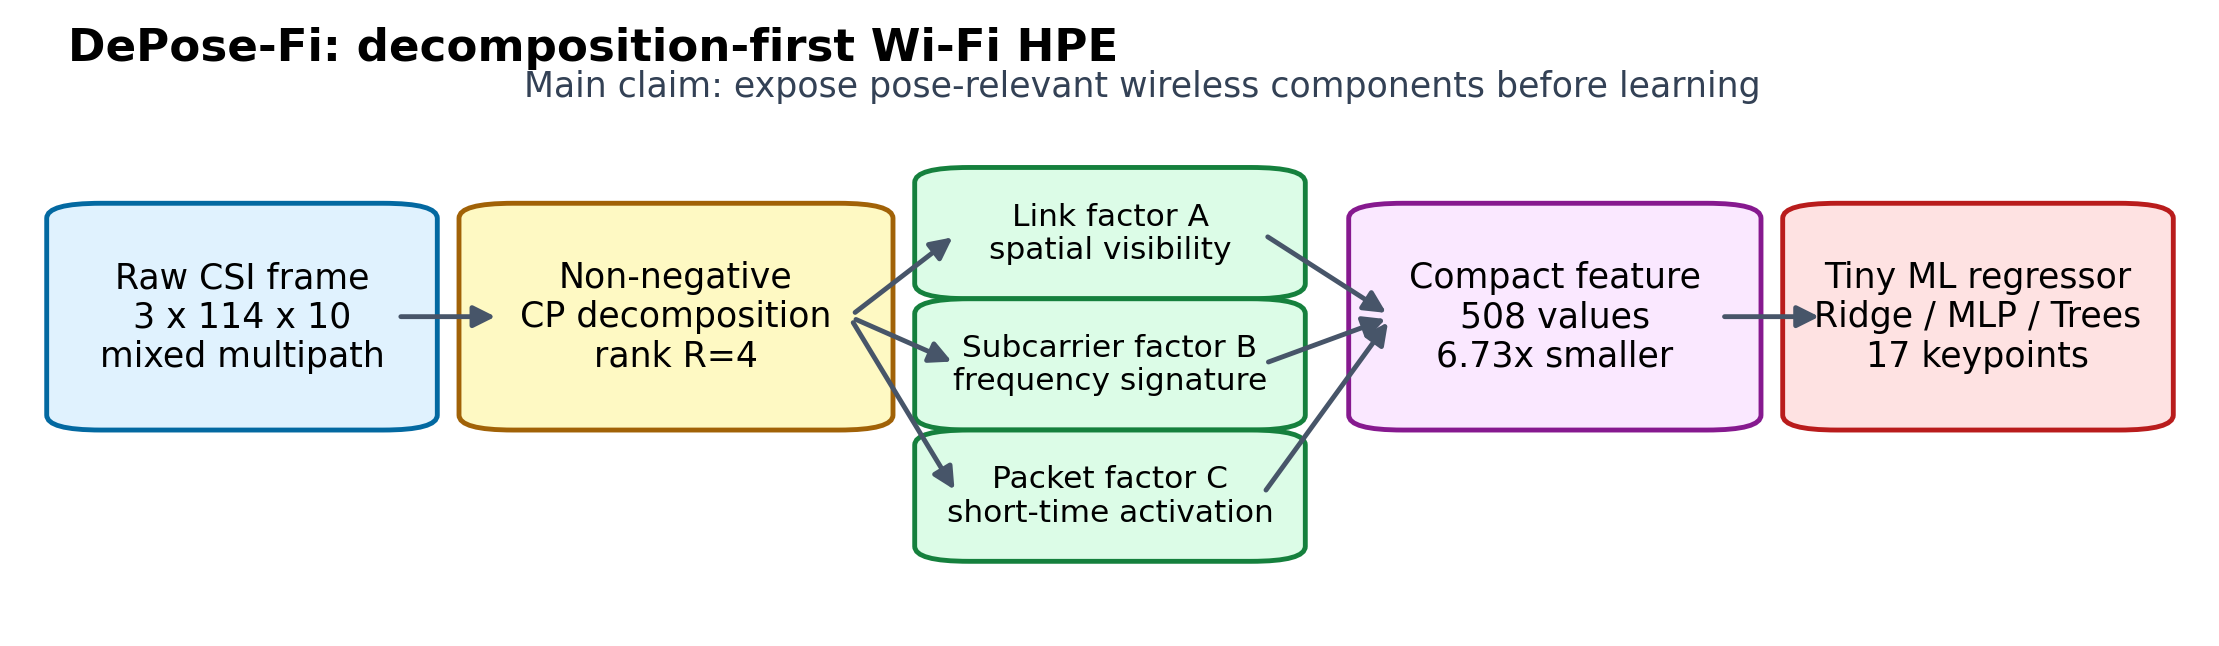
\includegraphics[width=0.95\linewidth]{figures/fig1_overview.pdf}
\caption{Overview of \method. Raw CSI is decomposed into link, subcarrier, and packet factors, then fused by a tiny component-adaptive predictor for pose estimation.}
\label{fig:overview}
\end{figure*}

\section{CSI Decomposition}

\subsection{Why CP Decomposition?}

Several decomposition choices are possible. PCA/SVD gives low-rank projections but introduces negative factors and poor physical interpretability. Matrix NMF gives non-negative parts but destroys CSI's multi-way structure by flattening the tensor. Tucker decomposition preserves modes but adds a dense core tensor, making components less direct to inspect. Neural autoencoders can be powerful, but they reintroduce a black-box representation learner.

We choose non-negative CP because it preserves CSI modes and produces interpretable rank-one components. Each component has a link signature, a frequency signature, and a packet activation. This is exactly the structure needed for a systems paper: the representation is compact, analyzable, and implementable.

\subsection{CP Formulation}

We approximate each CSI frame as
\begin{equation}
X(l,s,p)\approx
\hat{X}(l,s,p)=
\sum_{r=1}^{R}A(l,r)B(s,r)C(p,r),
\label{eq:cp}
\end{equation}
where $A\in\mathbb{R}_{+}^{L\times R}$, $B\in\mathbb{R}_{+}^{S\times R}$, and $C\in\mathbb{R}_{+}^{P\times R}$. The $r$-th component is
\begin{equation}
\mathcal{C}_r=A(:,r)\circ B(:,r)\circ C(:,r).
\end{equation}
The feature vector is
\begin{equation}
z=[A(:),B(:),C(:)].
\end{equation}
For rank $R=4$, this gives
\begin{equation}
R(L+S+P)=4(3+114+10)=508
\end{equation}
features, a $6.73\times$ reduction from the raw 3420-value CSI frame.

\begin{figure}[t]
\centering
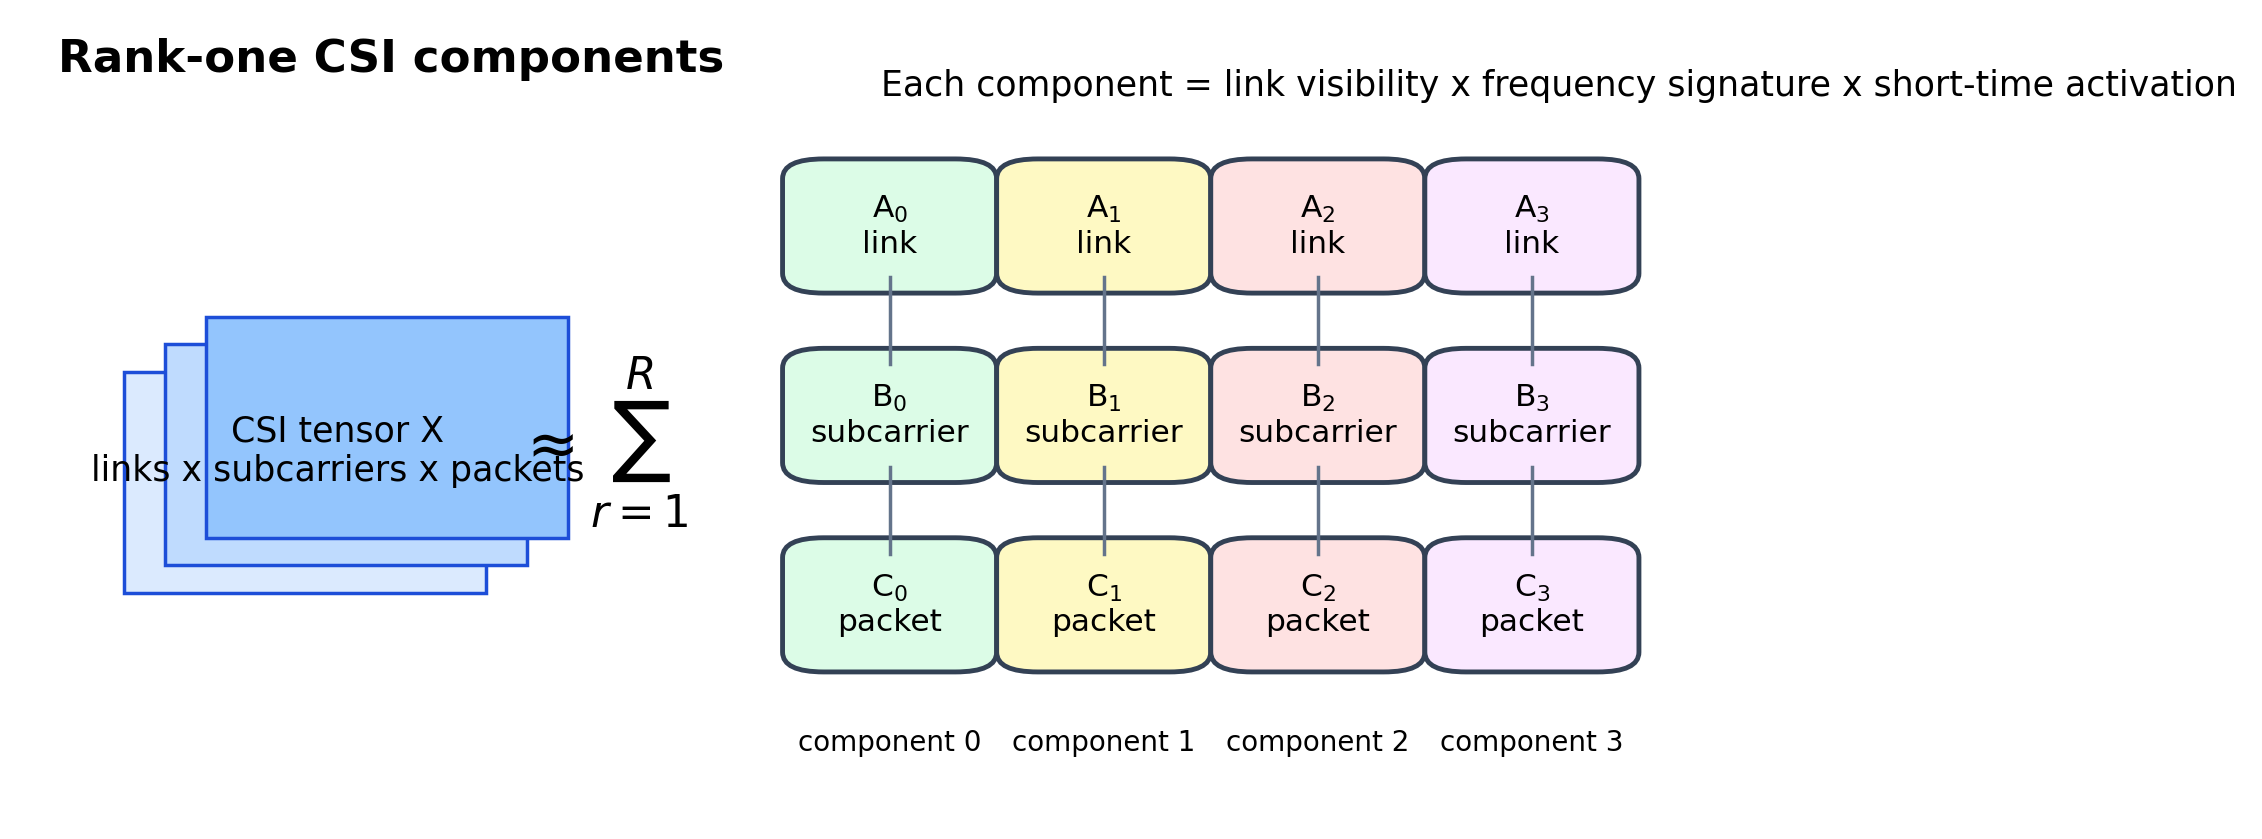
\includegraphics[width=0.95\linewidth]{figures/fig2_decomposition.pdf}
\caption{CP decomposes CSI into rank-one wireless components. Each component contains a link signature, a subcarrier signature, and a packet signature.}
\label{fig:decomposition}
\end{figure}

\subsection{Physical Interpretation}

The CP representation is useful because each factor corresponds to one physical axis of the wireless measurement. The link factor $A(:,r)$ indicates how strongly component $r$ is observed by each transmitter-receiver link. The subcarrier factor $B(:,r)$ captures the frequency-selective multipath signature of the component. The packet factor $C(:,r)$ captures short-time variation inside the frame. The component energy is
\begin{equation}
e_r=\|A(:,r)\|_2\|B(:,r)\|_2\|C(:,r)\|_2,
\end{equation}
and the normalized contribution is
\begin{equation}
\pi_r=\frac{e_r}{\sum_{j=1}^{R} e_j}.
\end{equation}
These quantities give a simple way to inspect whether the decomposition is dominated by one component or distributed across multiple components.

For pose estimation, the most important question is not whether CP perfectly reconstructs CSI. The important question is whether the factors expose pose-relevant structure. We therefore evaluate decomposition quality in three ways: reconstruction error, downstream PCK, and component removal. A component is considered useful only if removing it degrades pose estimation. This is stricter than showing a visually plausible factorization.

\subsection{Optimization}

The unsupervised reconstruction loss is
\begin{equation}
\mathcal{L}_{rec}=\|X-\hat{X}\|_F^2.
\end{equation}
Let $X_{(1)}$, $X_{(2)}$, and $X_{(3)}$ be mode unfoldings and $\odot$ the Khatri-Rao product. Multiplicative updates are:
\begin{align}
A &\leftarrow A\circ
\frac{X_{(1)}(B\odot C)}
{A((B^TB)\circ(C^TC))+\epsilon},\\
B &\leftarrow B\circ
\frac{X_{(2)}(A\odot C)}
{B((A^TA)\circ(C^TC))+\epsilon},\\
C &\leftarrow C\circ
\frac{X_{(3)}(A\odot B)}
{C((A^TA)\circ(B^TB))+\epsilon}.
\end{align}

The broader objective can include pose supervision:
\begin{equation}
\min_{A,B,C,\omega}
\mathcal{L}_{pose}(G_\omega(z),y)
+\lambda_r\mathcal{L}_{rec}
+\lambda_d\mathcal{L}_{div}
+\lambda_s\mathcal{L}_{sparse}
+\lambda_t\mathcal{L}_{smooth}.
\label{eq:future_objective}
\end{equation}
This paper uses the conservative unsupervised setting; Eq.~\ref{eq:future_objective} is the path toward a stronger pose-aware factorizer.

\subsection{Why Not Other Decompositions?}

The decomposition stage is not restricted to CP. A complete system could use PCA, SVD, matrix NMF, Tucker decomposition, ICA, sparse coding, or a learned autoencoder. We choose CP for this version because it gives the best trade-off among interpretability, compactness, and deployability.

PCA/SVD are fast and stable, but the resulting factors can be negative and are harder to map back to physical wireless energy. Matrix NMF keeps non-negativity, but it must flatten $X$ into a matrix; after flattening, link, subcarrier, and packet axes are mixed. Tucker decomposition is more expressive, but the core tensor creates interactions that are harder to explain and heavier to deploy. Autoencoders can learn powerful features, but they move the decomposition back into a black-box neural model, weakening the main claim of the paper. CP is not the only possible decomposition, but it is the cleanest first system point: it preserves all three CSI modes, produces compact factors, and keeps the representation inspectable.

\section{Selective Component-Adaptive Fusion}

The decomposition stage is useful only if the predictor respects the structure of the factors. A generic multilayer perceptron treats all CP coefficients as one unordered vector. This loses the distinction between link visibility, frequency-selective multipath, and packet-level variation. Selective component-adaptive fusion (S-AFF) is designed to preserve this structure while remaining small enough for edge deployment.

\subsection{Mode-Specialized Encoders}

S-AFF processes the three factor modes separately:
\begin{align}
h_A &= E_A(A),\\
h_B &= E_B(B),\\
h_C &= E_C(C).
\end{align}
The link branch $E_A$ is small because $A\in\mathbb{R}^{3\times R}$ has only three links. The subcarrier branch $E_B$ is the dominant branch because $B\in\mathbb{R}^{114\times R}$ contains frequency-selective multipath signatures. The packet branch $E_C$ captures short-time variation from $C\in\mathbb{R}^{10\times R}$. In our implementation, $E_B$ uses the largest hidden width, while $E_A$ and $E_C$ remain compact. This architecture is not arbitrary: the factor ablation in Table~\ref{tab:factor} shows that the subcarrier mode carries the strongest pose signal.

For each mode $M\in\{A,B,C\}$, the branch encoder has the form
\begin{equation}
h_M=\sigma(W_{M,2}\sigma(W_{M,1}\mathrm{vec}(M)+b_{M,1})+b_{M,2}),
\end{equation}
where $\sigma$ is ReLU. This keeps S-AFF easy to export because it uses only dense layers, lightweight one-dimensional convolutions, pooling, and pointwise nonlinearities.

\subsection{Selective Expert Fusion}

The first AFF design mixed only the three branch predictions. However, a frame may not need all branches: the subcarrier factor alone may be sufficient when frequency-selective multipath is highly informative, while a fused representation may be better when multiple modes agree. S-AFF therefore preserves the original branch embeddings and adds an explicit fused embedding:
\begin{equation}
h_F=E_F([h_A,h_B,h_C]).
\end{equation}
It then predicts four candidate poses:
\begin{align}
\hat{y}_A &= P_A(h_A),&
\hat{y}_B &= P_B(h_B),\\
\hat{y}_C &= P_C(h_C),&
\hat{y}_F &= P_F(h_F).
\end{align}
The gate is computed per sample:
\begin{equation}
\alpha=\mathrm{softmax}\left(\frac{W_g[h_A,h_B,h_C]+b_g}{\tau}\right),
\label{eq:aff_gate}
\end{equation}
where $\alpha_A+\alpha_B+\alpha_C+\alpha_F=1$ and $\tau$ is a temperature. The final pose is:
\begin{equation}
\hat{y}=
\alpha_A \hat{y}_A+
\alpha_B \hat{y}_B+
\alpha_C \hat{y}_C+
\alpha_F \hat{y}_F.
\label{eq:aff_pose}
\end{equation}
Eq.~\ref{eq:aff_gate} gives S-AFF a sample-dependent mechanism. It can select a single mode when one factor is sufficient, or select the fused expert when the pose evidence is distributed across factors. This is more appropriate for CP factors than uniform averaging because CP has already separated CSI into physically distinct modes.

\subsection{Gate Sharpening Loss}

A softmax gate can become uninformative if it assigns nearly uniform weights to all branches. Uniform gates are undesirable here because the factor ablation shows that the three modes do not carry equal pose information. We therefore add a sharpening term that minimizes gate entropy:
\begin{equation}
\mathcal{L}_{sharp}
=
\frac{1}{N}\sum_{i=1}^{N}
\left(
-\sum_{m\in\{A,B,C,F\}}
\alpha_{i,m}\log(\alpha_{i,m}+\epsilon)
\right).
\end{equation}
The S-AFF training objective is:
\begin{equation}
\mathcal{L}
=
\mathcal{L}_{pose}
\lambda_{sharp}\mathcal{L}_{sharp}.
\end{equation}
This loss encourages decisive gates, but it does not hard-code which branch should win. The winning branch is still learned from data. In our full-MM-Fi experiment, the learned gate chooses the subcarrier expert for 46.0\% of test frames and the fused expert for 54.0\%, with negligible probability assigned to link-only or packet-only experts. This matches the factor ablation: subcarrier structure is dominant in the single-frame protocol, but a fused representation is still useful for many frames.

\subsection{Why S-AFF Is a Contribution}

S-AFF is not meant to be a large accuracy-maximizing backbone. Its role is to make the decomposition deployable. The design has three properties that fit our systems goal.

\textbf{First, S-AFF is decomposition-aware.}
The architecture matches the CP structure. Link, subcarrier, and packet factors are not mixed until after each mode has been encoded.

\textbf{Second, S-AFF is selective and inspectable.}
The gate $\alpha$ can be logged at runtime to determine whether a prediction is driven by one factor mode or by the fused expert. The average maximum gate weight is 0.817 on the MM-Fi test set, showing that the model learns decisive routing rather than near-uniform averaging.

\textbf{Third, S-AFF is hardware-friendly.}
S-AFF uses dense layers, lightweight one-dimensional convolutions, ReLU, pooling, and softmax. These operations are supported by TorchScript, ONNX Runtime, TensorRT, and CPU vector libraries. This is why S-AFF is preferable to ExtraTrees despite similar offline accuracy: S-AFF maps cleanly to deployment runtimes, while a large tree ensemble produces irregular branch-heavy inference.

The design is inspired by WiDeFus's adaptive fusion principle~\cite{widefus2026}, but the adaptation is nontrivial. WiDeFus fuses frequency, time, and spatial features for activity classification. \method\ fuses CP-derived link, subcarrier, and packet factors for continuous 17-keypoint pose regression, preserves single-factor experts, and uses a sharpening loss to avoid weak uniform fusion.

\section{Implementation}

The CP solver uses rank $R=4$ and 10 multiplicative-update iterations for the main experiments. CSI amplitudes are loaded from MM-Fi MATLAB files, invalid values are replaced, and each frame is min-max normalized. The CP feature extractor outputs 508 features. S-AFF has 64.9K parameters and uses approximately 2.89M FLOPs per frame including CP extraction. CNN and ExtraTrees are implemented as comparison baselines: CNN tests whether local convolution over component maps improves accuracy, while ExtraTrees estimates an upper bound for nonlinear information in the decomposed features.

\subsection{CSI Preprocessing}

Each MM-Fi frame is a CSI amplitude tensor with shape $3\times114\times10$. Infinite values are treated as missing and replaced by the mean of valid entries in the corresponding packet slice. Each frame is min-max normalized:
\begin{equation}
\tilde{X}=\frac{X-\min(X)}{\max(X)-\min(X)+\epsilon}.
\end{equation}
This simple normalization is used intentionally because it is easy to reproduce on edge devices.

\subsection{Feature Extraction Cost}

For $L=3$, $S=114$, $P=10$, and $R=4$, one CP update iteration costs approximately 46.6K MACs. With 10 iterations, CP extraction costs approximately 466K MACs, or 0.93M FLOPs. S-AFF prediction costs approximately 0.98M MACs, or 1.96M FLOPs. Thus, the full CP+S-AFF pipeline costs approximately 2.89M FLOPs per frame.

\subsection{Model Export Path}

S-AFF is composed of standard neural operators: linear layers, 1D convolutions, pooling, ReLU, and softmax. This makes it portable to common deployment stacks. For Raspberry Pi, the target path is ONNX Runtime or TorchScript CPU inference. For Jetson Nano, TensorRT or TorchScript can be used. The CP stage can initially run as optimized NumPy/C++ code; a later version can replace iterative CP with a learned feed-forward factor extractor if CP becomes the latency bottleneck.

\section{Experimental Setup}

\subsection{Dataset and Protocol}

We evaluate on the full MM-Fi dataset~\cite{mmfi2023} using the HPE-Li frame-level protocol3 setting. The dataset contains 320,760 Wi-Fi CSI frames. The reproduced split gives 224,532 training frames and 96,228 validation/test frames; we use 48,114 held-out frames for test. PCK follows HPE-Li's MM-Fi implementation, where 2D keypoint error is normalized by the torso distance between keypoints 1 and 11.

To test whether the decomposition-first design generalizes beyond MM-Fi, we also evaluate on Person-in-WiFi 3D~\cite{personwifi3d2024}. This dataset targets 3D pose estimation from complex CSI with shape $3\times3\times30\times20$ and is therefore substantially different from the MM-Fi frame protocol. We evaluate two adaptations. First, for the native mixed-person split, we reshape CSI into a $9\times60\times20$ amplitude-plus-sanitized-phase tensor, apply rank-16 CP, and replace the fixed pose head with a lightweight query S-AFF head. Second, motivated by the stronger amplitude/phase separation required by Person-in-WiFi 3D-style 3D pose data, we decompose amplitude and sanitized phase as separate $9\times30\times20$ tensors with rank-24 CP, process them with two S-AFF streams, and learn a stream gate before query decoding. We evaluate this dual-stream CP adaptation on the single-person protocol used by recent Person-in-WiFi 3D comparisons. Training uses permutation/set matching over valid people, L1 pose loss, confidence/count supervision, a soft bone-length regularizer, and the S-AFF gate-sharpening loss.

\subsection{Baselines}

We compare mean pose, raw-statistic features, CP features with several predictors, and HPE-Li's reported result. Raw statistics use mode-wise means and standard deviations. CP variants use the decomposed factor vector. ExtraTrees is included only as an analysis baseline; it is not considered deployment-friendly.

\subsection{Metrics}

We report PCK$_{50}$, PCK$_{40}$, PCK$_{30}$, PCK$_{20}$, PCK$_{10}$, and MPJPE. PCK uses the HPE-Li MM-Fi implementation: predicted and ground-truth 2D keypoints are compared after normalization by the torso distance between keypoints 1 and 11. We also report parameters and FLOPs for deployment-oriented variants.

\section{Results}

\subsection{Main Accuracy}

\begin{table*}[t]
\centering
\caption{Full MM-Fi protocol-3 frame-level results.}
\label{tab:main}
\begin{tabular}{lrrrrrr}
\toprule
Method & PCK$_{50}$ & PCK$_{40}$ & PCK$_{30}$ & PCK$_{20}$ & PCK$_{10}$ & MPJPE \\
\midrule
Mean pose & 73.10 & 62.36 & 46.92 & 27.45 & 9.51 & 0.246 \\
Raw stats + Ridge & 80.12 & 71.17 & 58.14 & 39.06 & 14.52 & 0.219 \\
Raw stats + MLP64 & 82.14 & 74.74 & 63.43 & 44.69 & 17.37 & 0.208 \\
Raw stats + ExtraTrees & 81.99 & 74.38 & 63.68 & 47.27 & 21.22 & 0.204 \\
CP + MLP64 & 82.37 & 75.09 & 64.13 & 46.24 & 18.37 & 0.209 \\
CP + AFF & 83.45 & 76.55 & 66.00 & 48.64 & 20.70 & 0.200 \\
CP + CNN & \textbf{83.57} & \textbf{76.88} & \textbf{66.62} & 49.62 & 21.50 & 0.198 \\
CP + ExtraTrees & 83.32 & 76.34 & 66.20 & 50.40 & \textbf{24.01} & \textbf{0.197} \\
CP + S-AFF & 83.40 & 76.76 & \textbf{66.85} & \textbf{50.80} & 23.42 & 0.198 \\
HPE-Li reported & 85.12 & 78.18 & 68.22 & 52.07 & -- & -- \\
\bottomrule
\end{tabular}
\end{table*}

CP improves nonlinear predictors over raw-statistic features. CP+S-AFF is the proposed practical model: it achieves 50.80\% PCK$_{20}$ with 64.9K parameters. It improves over the original AFF by 2.16 PCK$_{20}$ points, exceeds CP+CNN and CP+ExtraTrees at the strict PCK$_{20}$ threshold, and remains much smaller than HPE-Li.

\begin{figure}[t]
\centering
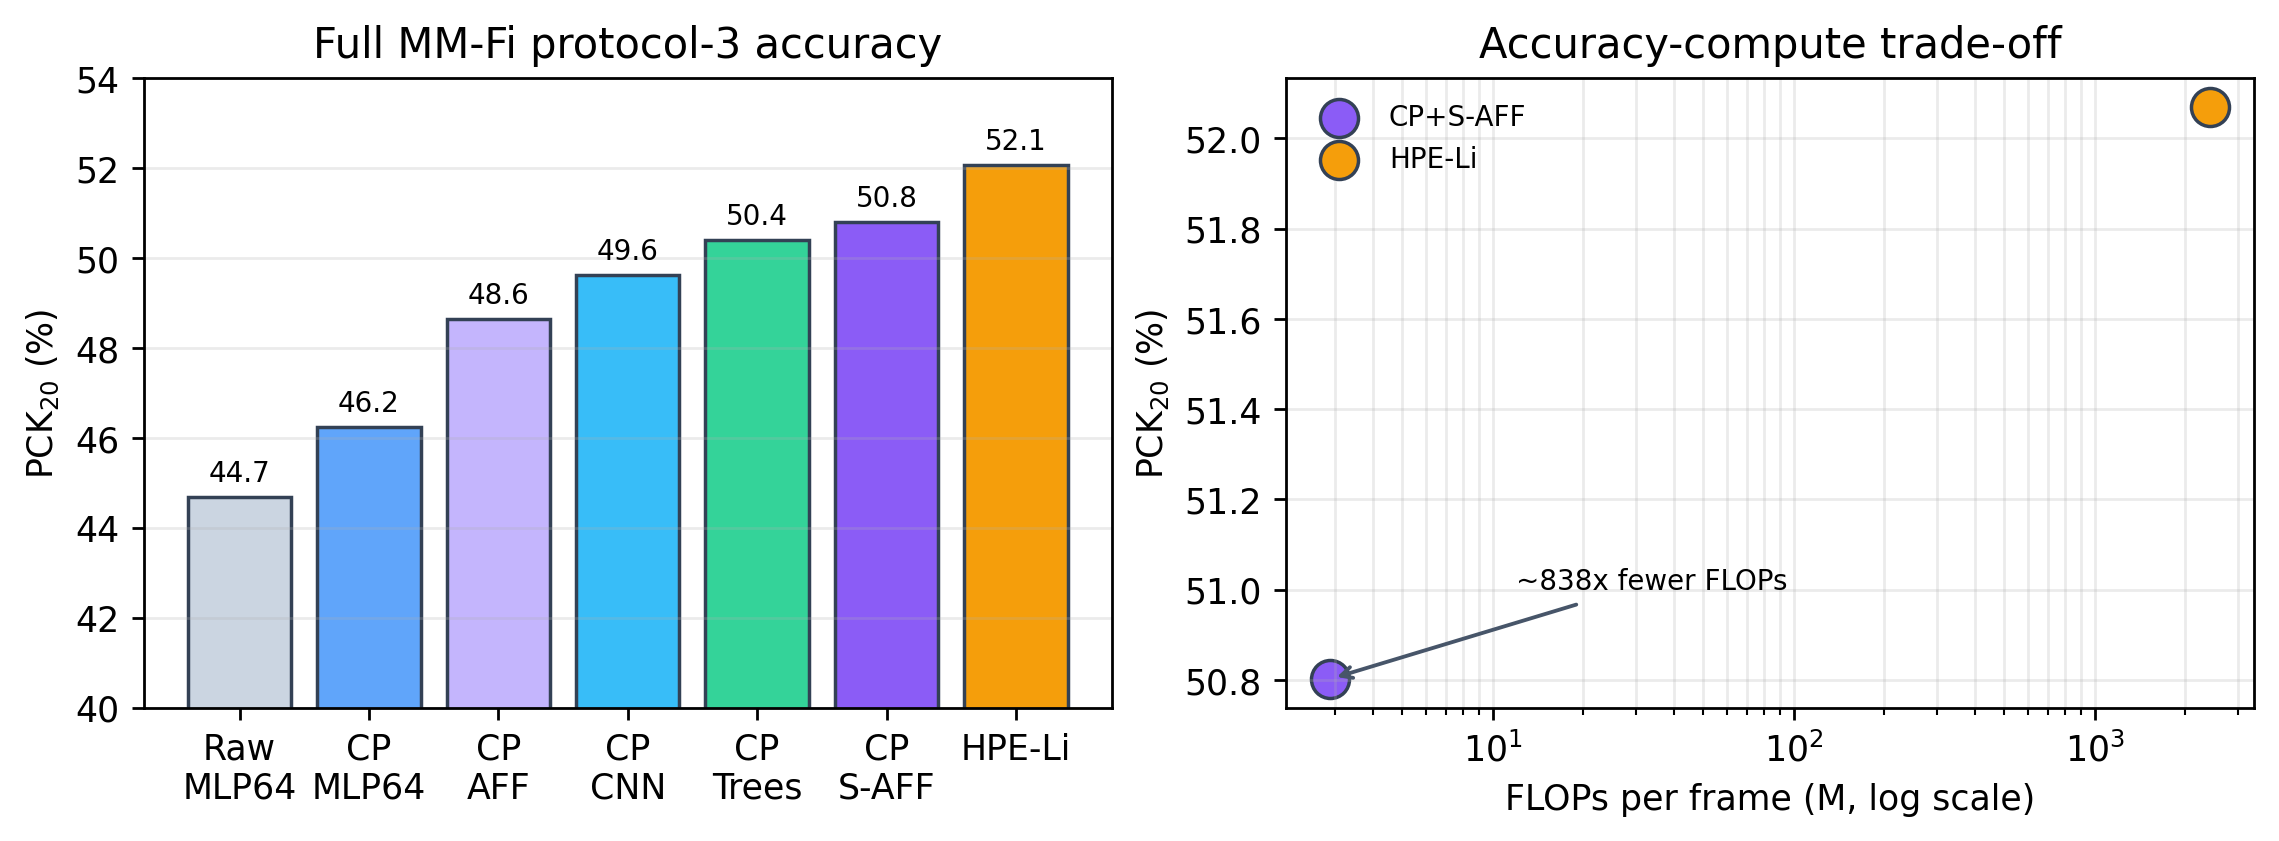
\includegraphics[width=0.95\linewidth]{figures/fig6_full_results_complexity.pdf}
\caption{Accuracy-complexity trade-off on full MM-Fi protocol3. CP+S-AFF is the best strict-threshold CP variant while remaining much smaller than HPE-Li.}
\label{fig:accuracy_complexity}
\end{figure}

\subsection{Cross-Dataset Adaptation to Person-in-WiFi 3D}

\begin{table}[t]
\centering
\caption{Cross-dataset adaptation on Person-in-WiFi 3D. Lower MPJPE is better.}
\label{tab:piw3d}
\begin{tabular}{lrrrr}
\toprule
Method & Params & MPJPE & PCK$_{100}$ & PCK$_{150}$ \\
\midrule
Mean pose, mixed-person & 0 & 1010.36 & 0.78 & 2.03 \\
CP + fixed S-AFF, mixed-person & 442.7K & 263.99 & 12.89 & 26.91 \\
CP + query S-AFF, mixed-person & 364.6K & 188.94 & 32.04 & 52.16 \\
CP + query S-AFF, 1P only & 943.6K & 113.72 & 65.25 & 78.60 \\
Dual CP + query S-AFF, 1P only & 1.70M & \textbf{83.82} & \textbf{76.01} & \textbf{86.10} \\
\bottomrule
\end{tabular}
\end{table}

Table~\ref{tab:piw3d} shows that the decomposition-first representation is not restricted to MM-Fi. On the native Person-in-WiFi 3D mixed-person split, CP+fixed S-AFF already improves over the mean-pose baseline, but its fixed three-slot output head is mismatched to the dataset's variable-person setting. Replacing only the output head with query S-AFF reduces MPJPE by 75.05 mm and more than doubles PCK$_{150}$. For the true single-person protocol, the same query S-AFF design reaches 113.72 mm. Separating amplitude and phase before CP improves the result further to 83.82 mm. This validates the central design lesson for Person-in-WiFi 3D-style datasets: amplitude and phase have different statistics and should be decomposed by separate CP streams rather than compressed into one amplitude-plus-phase tensor before fusion.

\begin{table}[t]
\centering
\caption{Person-in-WiFi 3D single-person adaptation sweep.}
\label{tab:piw3d_sweep}
\begin{tabular}{lrr}
\toprule
Variant & Params & MPJPE \\
\midrule
Combined CP + query S-AFF & 943.6K & 113.72 \\
Temporal CP smoothing & 943.6K & 202.85 \\
Learned temporal CP mixer & 1.34M & 242.68 \\
Dual CP, rank 16 & 1.68M & 92.16 \\
Dual CP, rank 24 & 1.70M & \textbf{83.82} \\
\bottomrule
\end{tabular}
\end{table}

Table~\ref{tab:piw3d_sweep} summarizes the adaptation sweep. Naively averaging CP vectors across neighboring frames hurts, and a learned temporal mixer over independently factorized CP embeddings also underperforms. This suggests that CP component identities are not temporally stable enough for direct vector-level temporal smoothing. In contrast, separating amplitude and phase before CP consistently improves single-person 3D pose accuracy on the Person-in-WiFi 3D dataset. The best large model reaches 83.82 mm MPJPE with 1.70M parameters. We therefore use separate amplitude/phase CP streams as the preferred adaptation for 3D Person-in-WiFi-style data, while leaving full mixed-person dual-stream training as future work.

\begin{table}[t]
\centering
\caption{Person-in-WiFi 3D single-person deployment profiles. Cached inference reports S-AFF/query inference after CP features are extracted.}
\label{tab:piw3d_profiles}
\begin{tabular}{lrrr}
\toprule
Profile & Params & MPJPE & Cached inference \\
\midrule
Dual CP + S-AFF-S & 248.2K & 107.53 & 21.37 $\mu$s \\
Dual CP + S-AFF-M & 923.2K & 91.35 & 50.30 $\mu$s \\
Dual CP + S-AFF-L & 1.70M & \textbf{83.82} & 85.56 $\mu$s \\
\bottomrule
\end{tabular}
\end{table}

Table~\ref{tab:piw3d_profiles} gives the more deployment-oriented interpretation. Dual CP+S-AFF is not a single operating point; it provides a controllable accuracy-size family. The small profile is 8.6$\times$ smaller than WiFi-Mamba but sacrifices accuracy. The medium profile is 2.3$\times$ smaller than WiFi-Mamba and approximately matches the original Person-in-WiFi 3D transformer baseline. The large profile gives the best accuracy in our family. This profile behavior is a practical advantage of the decomposition-first design: the CP rank and S-AFF width expose explicit knobs for deployment constraints.

\begin{table}[t]
\centering
\caption{Single-person Person-in-WiFi 3D comparison with recent reported results. Lower MPJPE is better.}
\label{tab:piw3d_sota}
\begin{tabular}{lrr}
\toprule
Method & Params & MPJPE \\
\midrule
Person-in-WiFi 3D~\cite{personwifi3d2024} & 48.2M & 91.77 \\
WiFi-Mamba~\cite{wifimamba2026} & 2.14M & \textbf{76.75} \\
Dual CP + S-AFF-S (ours) & 248.2K & 107.53 \\
Dual CP + S-AFF-M (ours) & 923.2K & 91.35 \\
Dual CP + S-AFF-L (ours) & 1.70M & 83.82 \\
\bottomrule
\end{tabular}
\end{table}

Table~\ref{tab:piw3d_sota} positions the adapted single-person model against the recent Person-in-WiFi 3D literature. Dual CP+S-AFF-L improves over the original Person-in-WiFi 3D transformer baseline by 7.95 mm MPJPE while using 28.3$\times$ fewer parameters. However, it remains 7.07 mm behind WiFi-Mamba, while the parameter reduction relative to WiFi-Mamba is modest. Therefore, Person-in-WiFi 3D should not be read as a state-of-the-art accuracy claim. Instead, it is a stress test showing that the decomposition-first representation can transfer to 3D Wi-Fi pose and expose useful deployment profiles. In particular, S-AFF-M roughly matches the original Person-in-WiFi 3D baseline with 52.2$\times$ fewer parameters, and S-AFF-S provides an aggressively small 248.2K-parameter option. The main deployment win of \method\ remains the MM-Fi setting, where it approaches HPE-Li accuracy with orders-of-magnitude lower FLOPs.

\begin{table}[t]
\centering
\caption{Person-in-WiFi 3D breakdown by number of people.}
\label{tab:piw3d_people}
\begin{tabular}{lrrr}
\toprule
People/frame & Samples & MPJPE & PCK$_{100}$ \\
\midrule
1 person & 2586 & 128.96 & 51.58 \\
2 people & 3184 & 191.32 & 32.24 \\
3 people & 2054 & 260.77 & 23.64 \\
\bottomrule
\end{tabular}
\end{table}

The per-count breakdown in Table~\ref{tab:piw3d_people} also identifies the remaining challenge. Accuracy degrades as the number of people increases, indicating that multi-person ambiguity, not CP extraction alone, is the dominant failure mode on Person-in-WiFi 3D. This motivates future work on stronger query assignment, person-presence calibration, and pose-aware factor extraction while retaining the lightweight decomposition-first pipeline.

\subsection{Complexity}

\begin{table}[t]
\centering
\caption{Complexity of deployment-oriented variants. FLOPs include CP extraction.}
\label{tab:complexity}
\begin{tabular}{lrrr}
\toprule
Model & Params & FLOPs & PCK$_{20}$ \\
\midrule
CP + MLP64 & 35.9K & 1.00M & 46.24 \\
CP + AFF & 44.3K & 2.85M & 48.64 \\
CP + S-AFF & 64.9K & 2.89M & 50.80 \\
CP + CNN & 77.6K & 5.06M & 49.62 \\
HPE-Li & 1.66M & 2.42G & 52.07 \\
\bottomrule
\end{tabular}
\end{table}

CP+S-AFF reduces parameters by 26$\times$ and FLOPs by more than 838$\times$ compared with HPE-Li. This is the core systems contribution: the model is not merely smaller in simulation, but structurally easier to deploy.

\subsection{Selective Fusion Behavior}

\begin{table}[t]
\centering
\caption{S-AFF gate behavior on the MM-Fi test set. The sharpened gate is decisive and mostly chooses either the dominant subcarrier expert or the fused expert.}
\label{tab:gate}
\begin{tabular}{lr}
\toprule
Gate statistic & Value \\
\midrule
Mean gate entropy & 0.401 \\
Mean maximum gate weight & 0.817 \\
Choose link expert & 0.00\% \\
Choose subcarrier expert & 46.04\% \\
Choose packet expert & 0.00\% \\
Choose fused expert & 53.96\% \\
\bottomrule
\end{tabular}
\end{table}

Table~\ref{tab:gate} shows why the selective fusion mechanism is useful. The model does not average all branches uniformly. Instead, it learns that single-frame MM-Fi is mostly explained by the subcarrier factor or by a fused representation that includes the subcarrier factor. This agrees with the factor-mode ablation in Table~\ref{tab:factor}, where removing the subcarrier factor causes the largest PCK$_{20}$ drop.

\subsection{Component Evidence}

\begin{table}[t]
\centering
\caption{Component ablation using CP+ExtraTrees.}
\label{tab:component}
\begin{tabular}{lrr}
\toprule
Input & PCK$_{20}$ & Drop \\
\midrule
All components & 50.40 & 0.00 \\
Drop component 0 & 36.74 & -13.66 \\
Drop component 1 & 42.85 & -7.55 \\
Drop component 2 & 41.35 & -9.05 \\
Drop component 3 & 31.46 & -18.94 \\
\bottomrule
\end{tabular}
\end{table}

Removing any component hurts accuracy, showing that CP factors are not cosmetic. Factor-mode ablation further shows that removing the subcarrier factor drops PCK$_{20}$ by 24.90 points, confirming that frequency-selective multipath is the dominant pose carrier in frame-level MM-Fi.

\begin{table}[t]
\centering
\caption{Factor-mode ablation. The subcarrier factor is the dominant pose carrier.}
\label{tab:factor}
\begin{tabular}{lrr}
\toprule
Input & PCK$_{20}$ & Drop \\
\midrule
All factors & 50.40 & 0.00 \\
Drop link factor $A$ & 47.72 & -2.68 \\
Drop subcarrier factor $B$ & 25.50 & -24.90 \\
Drop packet factor $C$ & 50.14 & -0.26 \\
\bottomrule
\end{tabular}
\end{table}

\begin{figure}[t]
\centering
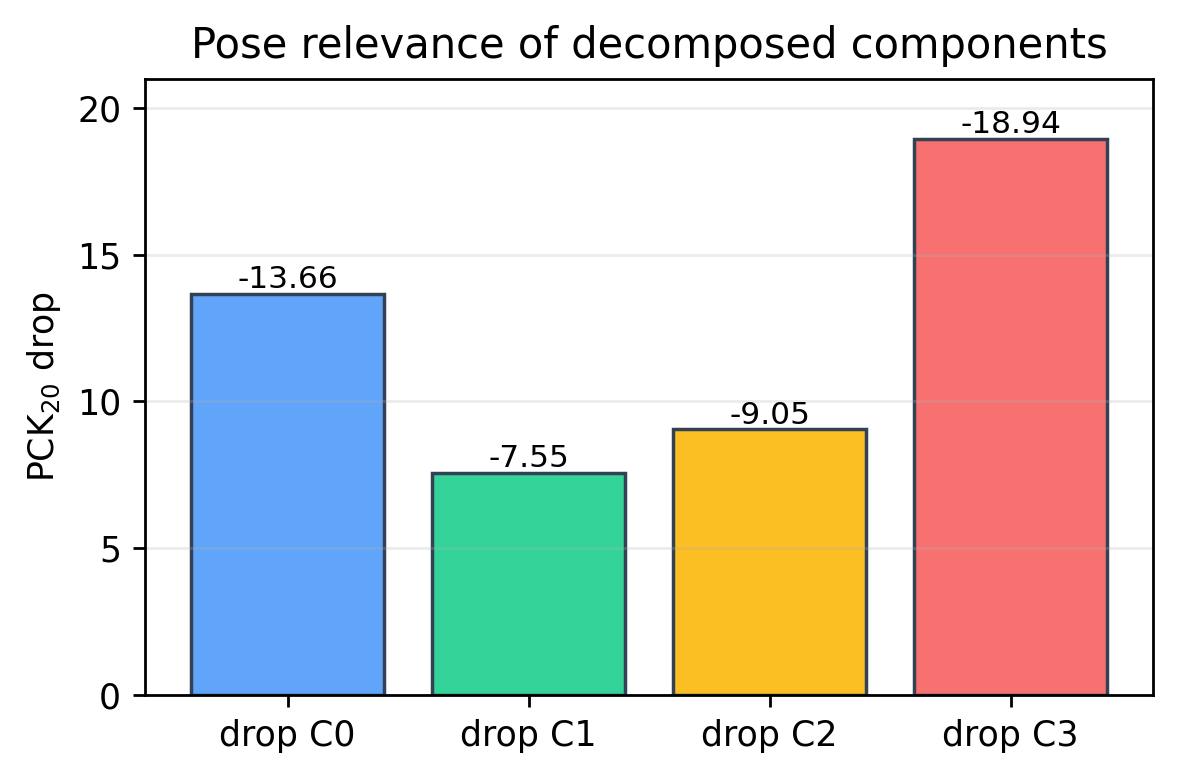
\includegraphics[width=0.95\linewidth]{figures/fig3_component_ablation.pdf}
\caption{Component ablation. Removing any CP component reduces PCK$_{20}$, showing that the factors carry complementary pose information.}
\label{fig:component_ablation}
\end{figure}

\begin{figure}[t]
\centering
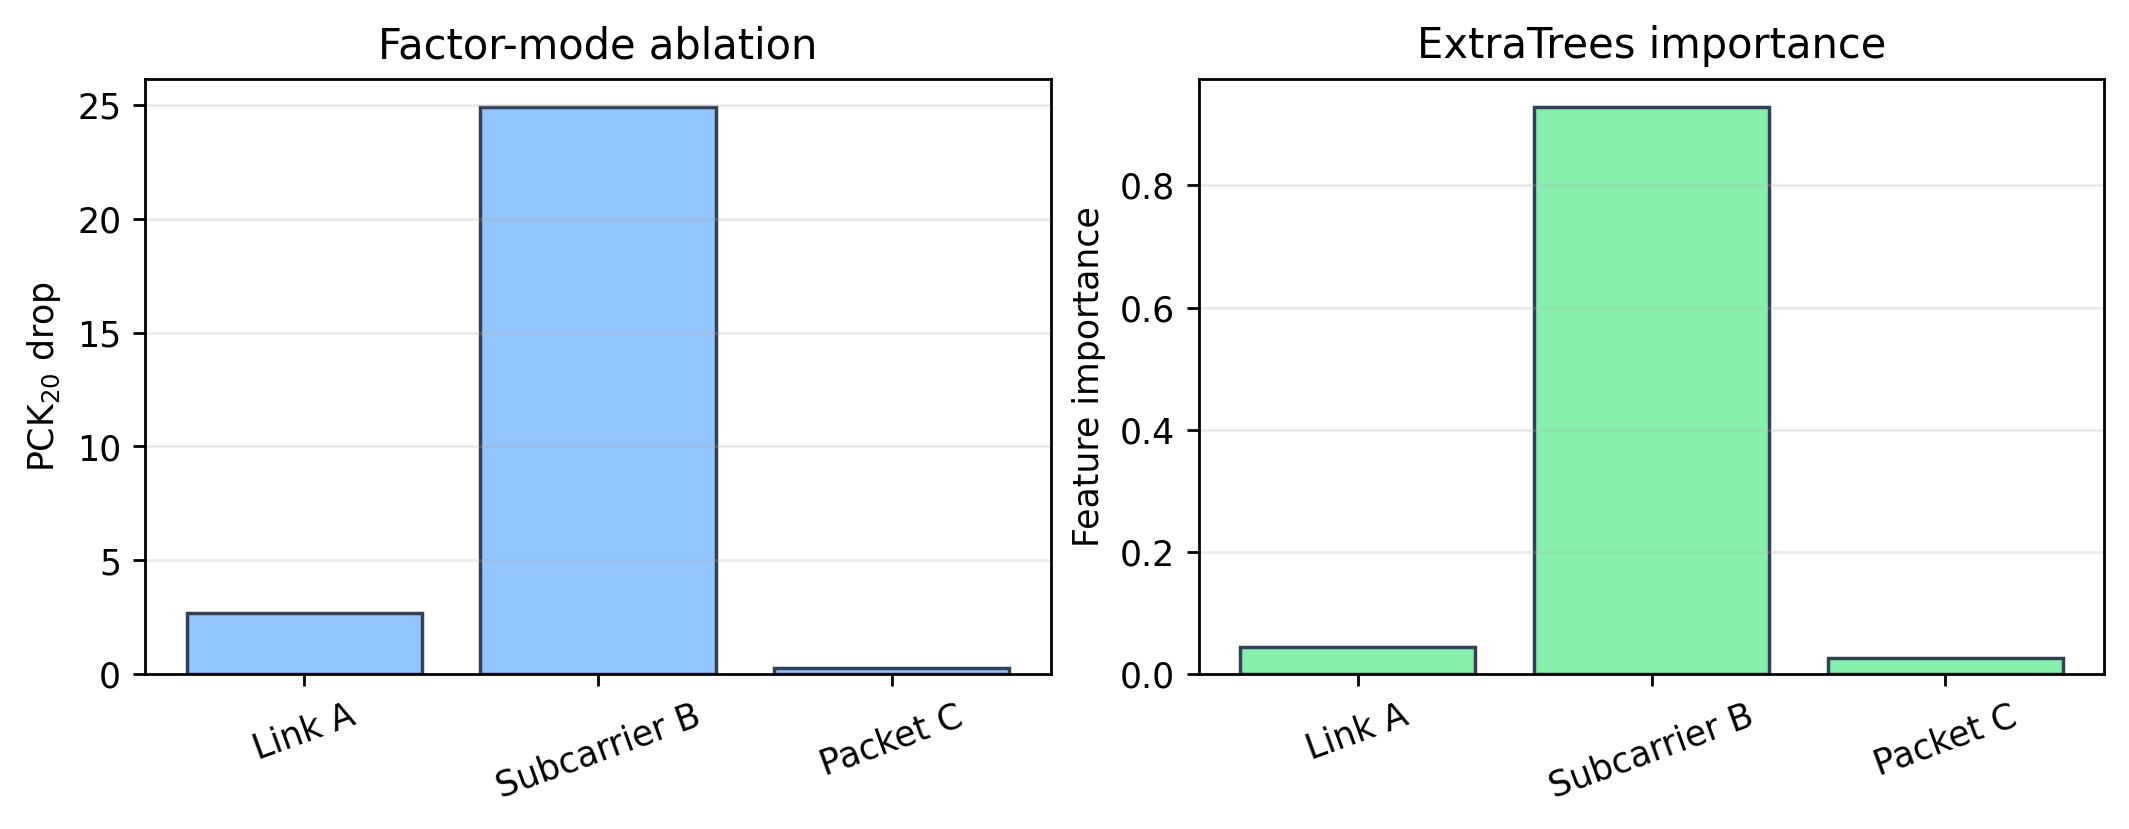
\includegraphics[width=0.95\linewidth]{figures/fig4_factor_importance.pdf}
\caption{Factor-mode importance. In single-frame MM-Fi, the subcarrier factor dominates because frequency-selective fading contains strong pose-dependent geometry.}
\label{fig:factor_importance}
\end{figure}

\subsection{Interpreting the Subcarrier Dominance}

The dominance of the subcarrier factor is not a failure of decomposition; it reveals how frame-level MM-Fi carries pose information. Each MM-Fi frame contains only 10 packets, so the packet axis provides limited temporal evidence. In contrast, each frame contains 114 subcarriers. These subcarriers sample frequency-selective fading caused by multipath geometry. Since human pose changes body-channel geometry, the subcarrier factor becomes the strongest carrier of pose information in a single-frame setting.

This result also guides the system design. S-AFF should not treat link, subcarrier, and packet factors equally. The subcarrier branch deserves more capacity, while the link and packet branches should remain small. The learned S-AFF gate confirms this: on the test set, it routes 46.0\% of frames to the subcarrier expert and 54.0\% to the fused expert, with almost no frames routed to link-only or packet-only experts. The ablation therefore provides both scientific evidence and an implementation rule.

\subsection{What CP Gives Beyond Accuracy}

Table~\ref{tab:main} shows that CP+Ridge is not better than raw-statistic Ridge. This is important. It means CP is not a magic linear feature transform. The value of CP appears when the predictor can use nonlinear interactions among decomposed factors. CP+MLP improves over raw-statistic MLP at strict thresholds, the original AFF improves further with a decomposition-aware architecture, and S-AFF improves again by making the gate selective rather than softly averaging all branches. Therefore, the right claim is not ``CP alone solves pose estimation.'' The right claim is: CP exposes structured components that a small nonlinear predictor can fuse more efficiently than learning from raw CSI directly.

This distinction matters for publication. If we sell only PCK, reviewers will ask why CP+Ridge is weak. If we sell decomposition as a systems abstraction, the evidence is stronger: CP gives interpretable factors, S-AFF uses those factors with 64.9K parameters, and ablation proves that individual components and factor modes matter.

\section{Edge Deployment Analysis}

\method\ is designed to make Wi-Fi HPE easier to deploy, not merely smaller on paper. We therefore analyze deployment friendliness from three angles: computational cost, runtime portability, and tuning flexibility.

\subsection{Accuracy--Cost Trade-off}

The main deployment result is that \method\ reaches a similar operating regime to HPE-Li with a much smaller inference budget. HPE-Li reports 52.07\% PCK$_{20}$ with 1.66M parameters and 2.42G FLOPs. CP+S-AFF reaches 50.80\% PCK$_{20}$ with 64.9K parameters and 2.89M FLOPs. Thus, \method\ sacrifices only 1.27 PCK$_{20}$ points while reducing parameters by 26$\times$ and FLOPs by more than 838$\times$.

This trade-off is the core systems result. For cloud inference, a 3.43-point accuracy gap may not be attractive. For edge inference, the compute reduction is large enough to change the deployment class of the model: from a neural HPE backbone that benefits from strong hardware acceleration to a tiny fusion predictor that can plausibly run on CPU-only devices.

\subsection{Deployment Friction}

Parameter count and FLOPs do not fully describe deployment difficulty. Some methods are small but hard to export; others require irregular runtime support. Table~\ref{tab:deployment_friction} summarizes deployment friction qualitatively.

\begin{table}[t]
\centering
\caption{Deployment-friendliness comparison.}
\label{tab:deployment_friction}
\begin{tabular}{lcccc}
\toprule
Method & Export & Custom ops & GPU need & Edge fit \\
\midrule
Transformer HPE & Medium & Possible & High & Weak \\
Graph HPE & Medium & Graph ops & Medium & Medium \\
CP + ExtraTrees & Weak & Branches & Low & Weak \\
CP + CNN & Strong & No & Low & Good \\
CP + S-AFF & Strong & No & Low & Strong \\
\bottomrule
\end{tabular}
\end{table}

S-AFF is favorable because it consists of dense layers, lightweight 1D convolutions, ReLU, pooling, and softmax. These operations are supported by standard edge inference stacks. ExtraTrees is competitive offline, but a large tree ensemble is less attractive for deployment because it requires many branch comparisons and has poorer vectorization behavior. This is why CP+ExtraTrees is used as an analysis baseline, while CP+S-AFF is the proposed deployable system.

\subsection{Controllable Compute Knobs}

\method\ also exposes explicit compute knobs through CP rank $R$ and iteration count $T$. Increasing $R$ gives more components; increasing $T$ improves factor convergence. Both increase computation predictably. This creates a family of deployment profiles:

\begin{table}[t]
\centering
\caption{Deployment profiles enabled by CP rank and iteration knobs.}
\label{tab:profiles}
\begin{tabular}{lcccl}
\toprule
Profile & Rank & Iters & Cost & Target \\
\midrule
SwiftPose-Fi-S & 2 & 5 & Lowest & Tiny CPU \\
SwiftPose-Fi-M & 4 & 10 & Medium & Edge CPU \\
SwiftPose-Fi-L & 6 & 15 & Higher & Edge GPU \\
\bottomrule
\end{tabular}
\end{table}

The current experiments evaluate the middle profile, SwiftPose-Fi-M, because it balances accuracy and cost. A complete deployment study should evaluate all three profiles on Raspberry Pi and Jetson Nano. This will let the system choose a profile based on device capability, latency target, or battery constraint.

\subsection{Hardware Experiment Design}

To prove hardware friendliness, the final paper should report direct measurements rather than only FLOPs. For each device, we should measure:
\begin{itemize}
    \item CSI preprocessing latency,
    \item CP decomposition latency,
    \item S-AFF inference latency,
    \item end-to-end frame latency,
    \item FPS,
    \item peak memory,
    \item serialized model size,
    \item CPU/GPU utilization,
    \item power and energy per frame when available.
\end{itemize}

The expected bottleneck is CP extraction. This is a useful engineering insight: S-AFF is already tiny, so future optimization can focus on CP kernels, warm-started CP, lower-rank profiles, or a learned feed-forward factor extractor. The deployment story therefore becomes concrete: decomposition makes the predictor tiny, and the remaining bottleneck is isolated and optimizable.

\section{Real-Device Validation Protocol}

The next step is to validate the deployment argument on real edge hardware. The protocol is straightforward and should be included before submission.

\textbf{Devices.}
Run CP+S-AFF on Raspberry Pi and Jetson Nano. Raspberry Pi represents a low-power CPU-only sensing gateway. Jetson Nano represents a small GPU-capable edge platform. Together, they cover the two practical deployment regimes for low-cost Wi-Fi sensing.

\textbf{Metrics.}
Report CSI preprocessing latency, CP decomposition latency, S-AFF inference latency, total frame latency, FPS, peak memory, average power, and energy per frame. Also report serialized model size and model load time. The key requirement is to separate CP latency from S-AFF latency so the bottleneck is visible.

\textbf{Baselines.}
Compare CP+S-AFF against CP+MLP64, the original CP+AFF, and CP+CNN on the same devices. HPE-Li should be included using its known FLOPs and parameters, and, if feasible, reproduced latency on the same hardware. ExtraTrees should not be treated as a deployment baseline; it is an analysis baseline.

\textbf{Expected bottleneck.}
S-AFF inference should be cheap. The likely bottleneck is iterative CP extraction. This does not weaken the system claim; it localizes the engineering bottleneck. If hardware profiling confirms this behavior, the optimization path is clear: accelerate CP kernels, warm-start factor updates, lower rank/iteration counts, or replace iterative CP with a learned feed-forward factor extractor.

\section{Discussion}

\textbf{Why S-AFF is the right deployable model.}
CNN is familiar and not the novelty. ExtraTrees is accurate but memory-heavy and branch-heavy. S-AFF is the right systems model because it is built around the decomposition: it separately processes link, subcarrier, and packet factors, preserves single-factor experts, and learns when to use a single expert or a fused expert. This gives us a story that is both algorithmically meaningful and implementation-friendly.

\textbf{What remains to be done.}
The current results are full-dataset but not yet hardware-measured. The next system experiment is to run CP+S-AFF on Raspberry Pi and Jetson Nano and report latency, FPS, memory, and power. The likely bottleneck is CP extraction, not S-AFF inference. A deployable version can optimize CP kernels or replace iterative CP with a learned feed-forward factor extractor.

\textbf{Why this is a bridge from simulation to practice.}
Many Wi-Fi HPE papers report accuracy, but practical deployment requires more than a good PCK table. A deployable system must have predictable compute, small memory, portable inference, and interpretable failure modes. \method\ moves in this direction by separating signal decomposition from pose fusion.

\section{Conclusion}

This paper presents \method, a decomposition-first Wi-Fi HPE system for practical edge deployment. \method\ decomposes CSI into link, subcarrier, and packet factors using CP decomposition, then fuses them with a tiny selective component-adaptive neural predictor. On full MM-Fi protocol3, CP+S-AFF approaches the accuracy regime of HPE-Li while reducing parameters by 26$\times$ and FLOPs by more than 838$\times$. On Person-in-WiFi 3D, adapting the S-AFF head to lightweight person queries improves mixed-person 3D pose estimation over a fixed-slot head, and separating amplitude/phase CP streams reaches 83.82 mm MPJPE on the single-person protocol, though it does not surpass the latest WiFi-Mamba result. Component ablation and cross-dataset adaptation show that the decomposed factors are strongly pose-relevant. These results support a practical direction for Wi-Fi HPE: decompose the wireless signal first, then deploy a compact fusion model on real hardware.

\bibliographystyle{IEEEtran}
\begin{thebibliography}{10}

\bibitem{personwifi2019}
F. Wang et al., ``Person-in-WiFi: Fine-grained person perception using WiFi,'' arXiv:1904.00276, 2019.

\bibitem{gopose2021}
M. Zhao et al., ``3D human pose estimation using WiFi signals,'' in \emph{Proc. IEEE/CVF ICCV Workshops}, 2021.

\bibitem{metafi2022}
Z. Zhao et al., ``MetaFi: Device-free pose estimation via commodity WiFi,'' arXiv:2208.10414, 2022.

\bibitem{mmfi2023}
Y. Yang et al., ``MM-Fi: Multi-modal non-intrusive 4D human dataset for versatile wireless sensing,'' arXiv:2305.10345, 2023.

\bibitem{personwifi3d2024}
F. Wang et al., ``Person-in-WiFi 3D: End-to-end multi-person 3D pose estimation with Wi-Fi,'' in \emph{Proc. IEEE/CVF CVPR}, 2024.

\bibitem{wifimamba2026}
Q.-A. N. Duc and K.-S. Wong, ``Interleaved selective state space models for efficient WiFi-based 3D multi-person pose estimation,'' \emph{Proc. ICML}, 2026.

\bibitem{hpeli2024}
T. D. Gian et al., ``HPE-Li: WiFi-enabled lightweight dual selective kernel convolution for human pose estimation,'' ECCV, 2024.

\bibitem{graphposefi2026}
Y. Chen, M. Qu, and S. Tang, ``Graph-based 3D human pose estimation using WiFi signals,'' 2026.

\bibitem{multidimfi2025}
Y. Zhang, X. Wang, and C. Wu, ``MultiDim-Fi: WiFi-based 3D human pose estimation via multi-dimensional transformer with staged attention,'' 2025.

\bibitem{efficientfi2023}
Y. Yang, C. Chen, and H. Zou, ``EfficientFi: Toward large-scale lightweight WiFi sensing via CSI compression,'' 2022.

\bibitem{litehar2022}
H. Salehinejad and S. Valaee, ``LiteHAR: Lightweight human activity recognition from WiFi signals with random convolution kernels,'' 2022.

\bibitem{sensefi2023}
Y. Yang, C. Chen, and H. Zou, ``SenseFi: A library and benchmark on deep-learning-empowered WiFi human sensing,'' 2023.

\bibitem{widefus2026}
W. Liu et al., ``WiDeFus: A Wi-Fi-based lightweight human activity recognition via CSI component decomposition and adaptive feature fusion,'' IEEE TCCN, 2026.

\bibitem{kolda2009}
T. G. Kolda and B. W. Bader, ``Tensor decompositions and applications,'' SIAM Review, 2009.

\end{thebibliography}

\end{document}
